
\subsubsection{P1: Scale Ordering with Diminishing Returns --- SUPPORTED}

\begin{table}[htbp]
\centering
\resizebox{\columnwidth}{!}{%
\begin{tabular}{llll}
\toprule
Scale & Accuracy & Cohen's Kappa & $\Delta$ from Previous \\
\midrule
7B & 58.5\% & 0.131 & --- \\
70B & 70.7\% & 0.394 & +12.2pp \\
Proprietary & 71.3\% & 0.396 & +0.6pp \\
\bottomrule
\end{tabular}
}
\end{table}

The diminishing returns ratio is 20.3:1 (12.2pp / 0.6pp). Kruskal-Wallis H=7.71, p=0.021, confirming that scale differences are statistically significant.

The $7B\rightarrow 70B$ transition captures approximately 95\% of the total scale benefit (12.2 of 12.8 percentage points). Cohen's Kappa indicates that 7B judges achieve only slight agreement ($\kappa$=0.131), while 70B and proprietary judges achieve fair agreement ($\kappa\approx 0.39-0.40)$.

\subsubsection{P2: Scale-Dependent Error Patterns --- SUPPORTED}

\begin{table*}[htbp]
\centering
\resizebox{\dimexpr 2\columnwidth+\columnsep\relax}{!}{%
\begin{tabular}{llllllll}
\toprule
Scale & Accuracy & FPR & FNR & TP & TN & FP & FN \\
\midrule
7B & 37.6\% & 74.8\% & 12.8\% & 143 & 165 & 491 & 21 \\
70B & 40.6\% & 69.2\% & 20.1\% & 131 & 202 & 454 & 33 \\
Proprietary & 45.9\% & 60.4\% & 29.3\% & 116 & 260 & 396 & 48 \\
\bottomrule
\end{tabular}
}
\end{table*}

Chi-square $\chi^{2}=45.78$, df=6, p=3.$27\times 10^{-8}$.

Key pattern: FPR decreases with scale (74.8\% $\rightarrow$ 69.2\% $\rightarrow$ 60.4\%) while FNR increases (12.8\% $\rightarrow$ 20.1\% $\rightarrow$ 29.3\%). Smaller models over-accept (high false positive rate); larger models under-accept (high false negative rate).

\begin{figure}[htbp]
\centering
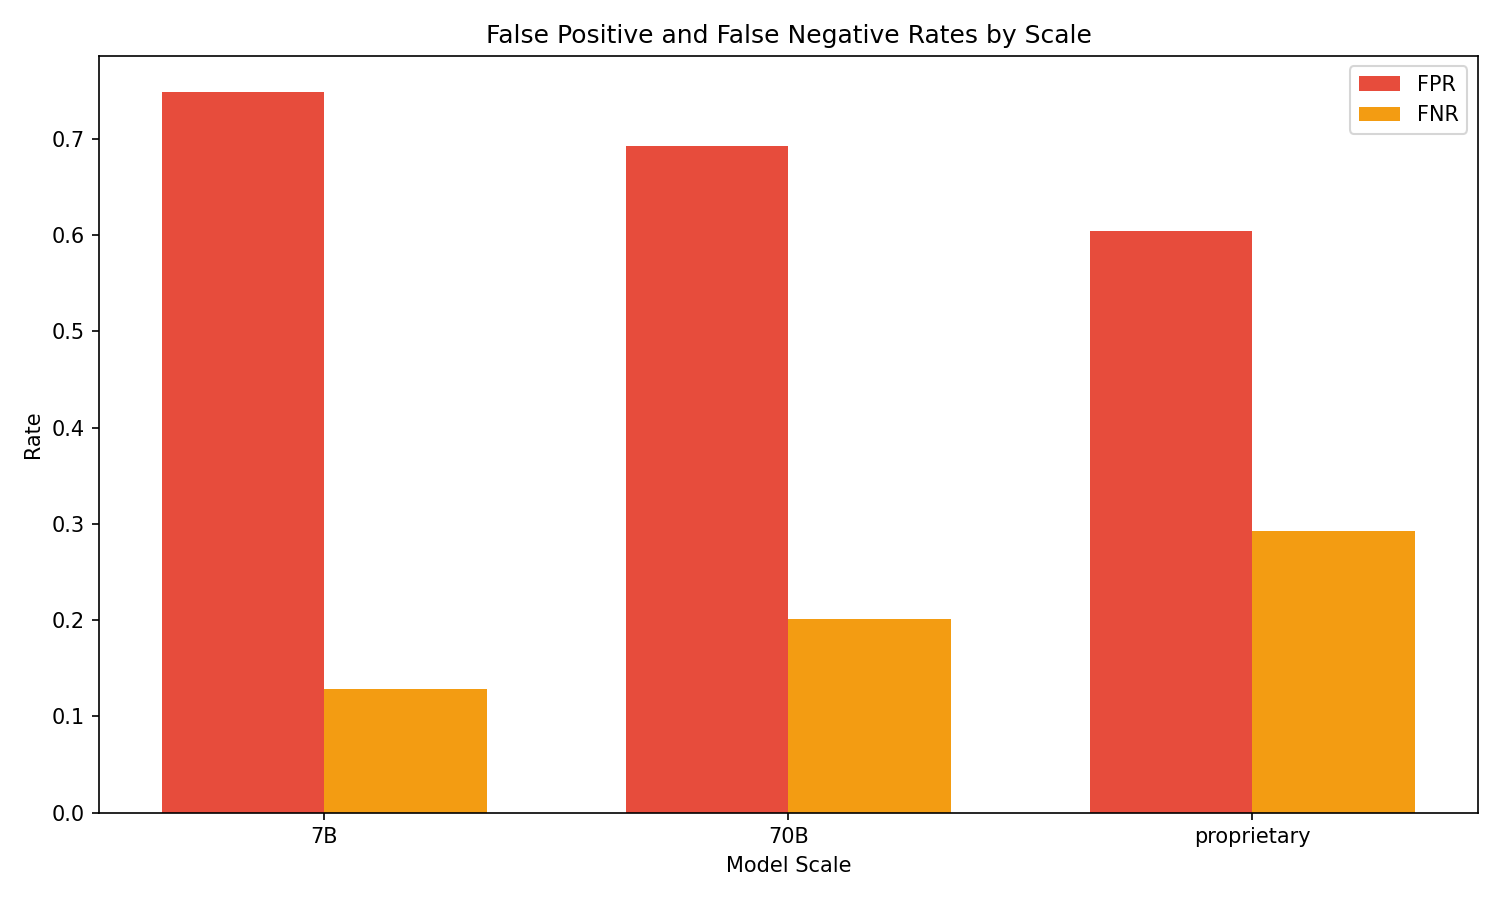
\includegraphics[width=\columnwidth]{figures/fp_fn_comparison.png}
\caption{FPR/FNR comparison across scales}
\label{fig:fp_fn_comparison}
\end{figure}

\subsubsection{P3: Ensemble Benefit --- FALSIFIED}

\begin{table}[htbp]
\centering
\resizebox{\columnwidth}{!}{%
\begin{tabular}{llll}
\toprule
Method & Accuracy & $\Delta$ vs Best Single & p-value \\
\midrule
Best single (Proprietary) & 45.85\% & --- & --- \\
AB1 (Simple majority) & 37.80\% & $-8.05$\% & 1.$45\times 10^{-6}$ \\
AB2 (Weighted majority) & 37.80\% & $-8.05$\% & 1.$45\times 10^{-6}$ \\
AB3 (Two-tier) & 45.85\% & 0.00\% & 1.00 \\
AB4 (Random) & 41.46\% & $-4.39$\% & 0.014 \\
\bottomrule
\end{tabular}
}
\end{table}

McNemar test confirms that ensemble voting is significantly worse than the best single judge (p=1.$45\times 10^{-6})$. The AB3 two-tier method (70B + proprietary only) matches but does not exceed proprietary alone, as tie-breaking defaults to the proprietary verdict.

The hypothesis that scale-diverse ensembles would outperform single judges by $\geq 3$\% is rejected. The observed degradation of 8.05\% is in the opposite direction from the predicted improvement.

\begin{figure}[htbp]
\centering
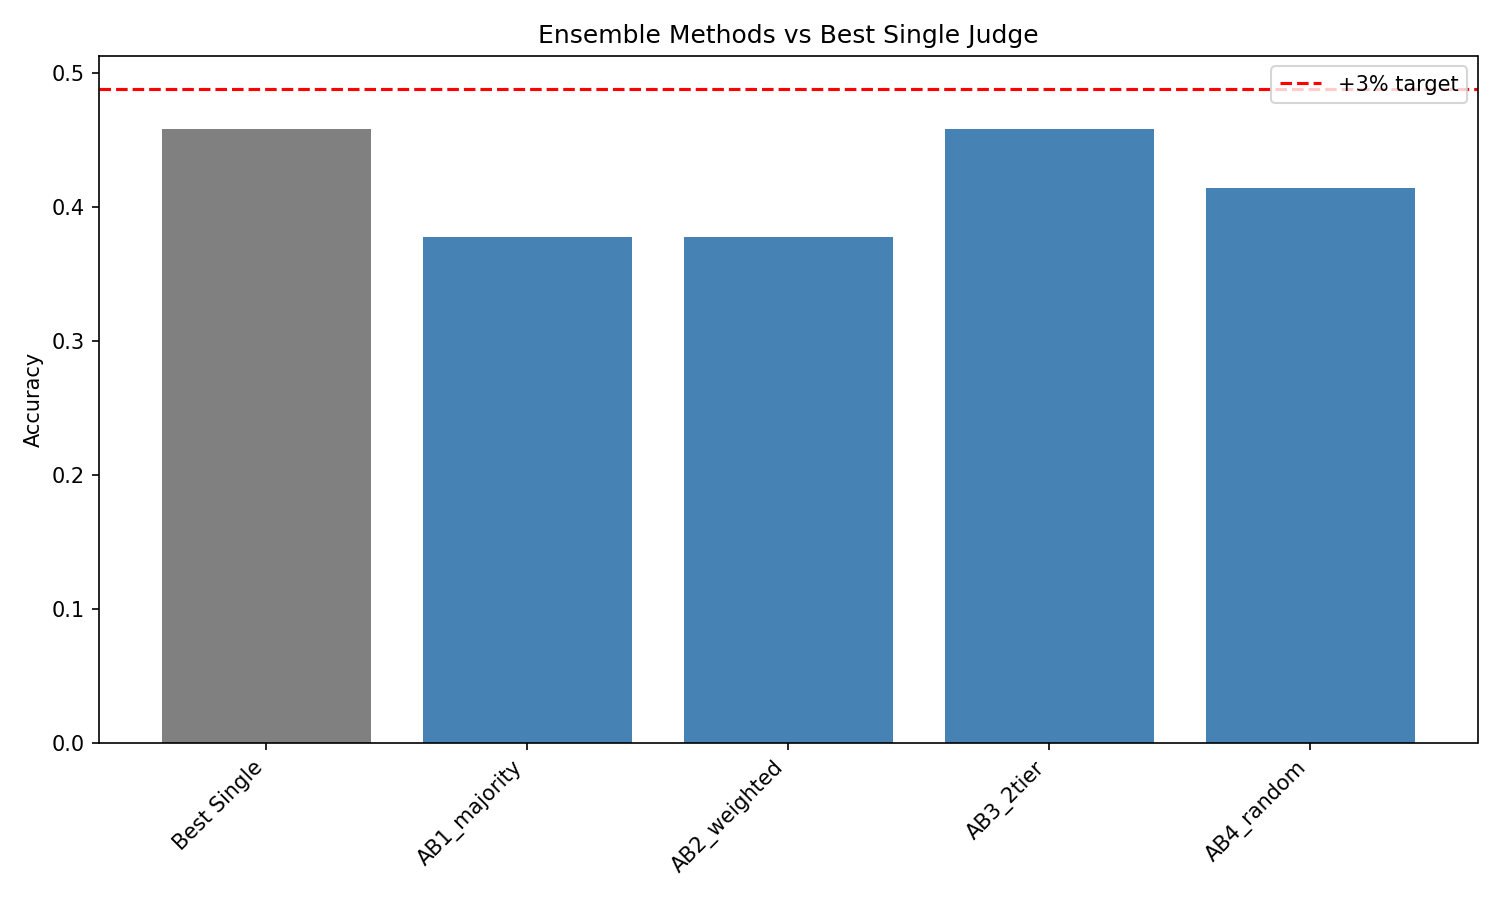
\includegraphics[width=\columnwidth]{figures/accuracy_comparison.png}
\caption{Accuracy comparison across methods}
\label{fig:accuracy_comparison}
\end{figure}

\subsubsection{P4: Unanimous Reliability --- FALSIFIED}

\begin{table}[htbp]
\centering
\resizebox{\columnwidth}{!}{%
\begin{tabular}{lll}
\toprule
Agreement Type & N & Accuracy \\
\midrule
Unanimous & 397 & 35.77\% \\
Split & 423 & 39.72\% \\
\bottomrule
\end{tabular}
}
\end{table}

Difference: $-3.95pp$ (opposite direction from +10\% threshold). Z-statistic=$-1.165$, p=0.878 (not significant).

The hypothesis that unanimous agreement signals higher reliability is rejected. Unanimous verdicts exhibit lower accuracy than split verdicts. The result, while directionally opposite to the hypothesis, is not statistically significant.

\begin{figure}[htbp]
\centering
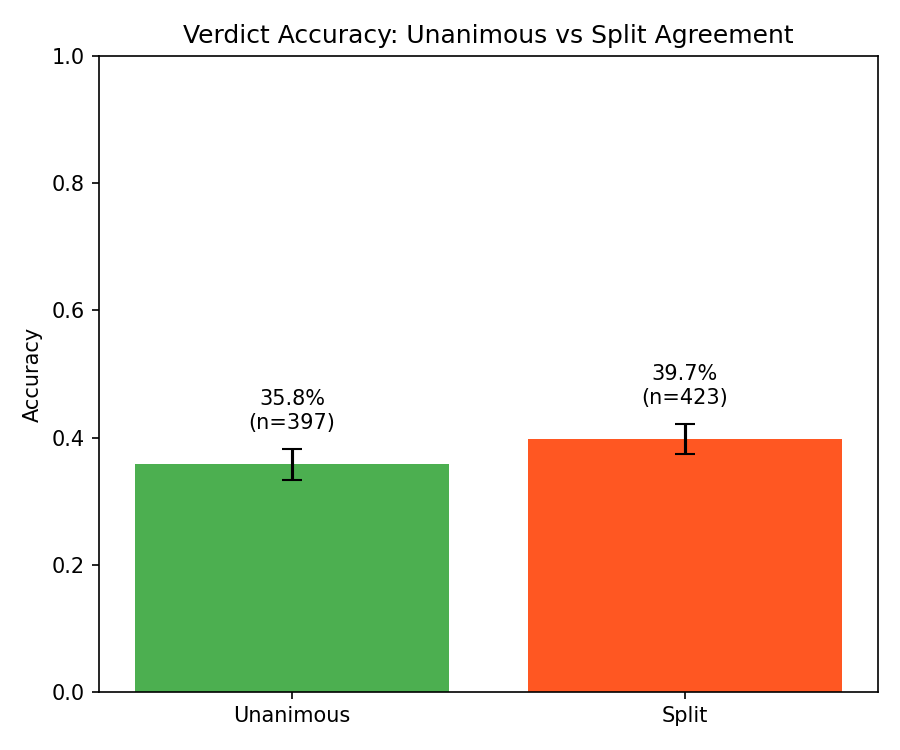
\includegraphics[width=\columnwidth]{figures/bar_chart.png}
\caption{Unanimous vs split accuracy}
\label{fig:bar_chart}
\end{figure}

